\documentclass[tikz,border=10pt]{standalone}
\begin{document}
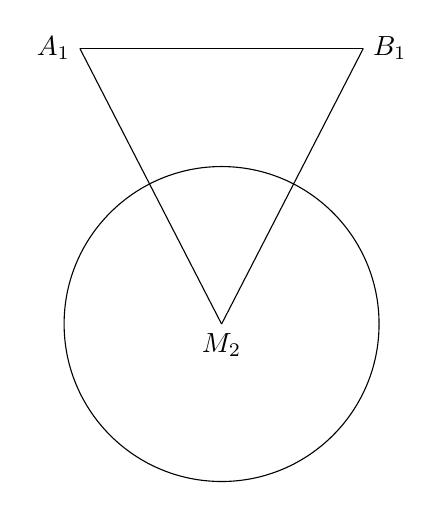
\begin{tikzpicture}
    \coordinate (A1) at (-1.8, 3.5);
    \coordinate (B1) at (1.8, 3.5);
    \coordinate (M2) at (0, 0);

    \draw (M2) circle (2);
    \draw (A1) -- (B1);
    \draw (A1) -- (M2);
    \draw (B1) -- (M2);

    \node[left] at (A1) {$A_1$};
    \node[right] at (B1) {$B_1$};
    \node[below] at (M2) {$M_2$};
\end{tikzpicture}
\end{document}
